\documentclass[a4paper,10pt]{article}
\usepackage[left=2.5cm,right=2.5cm,top=2.5cm,bottom=2.5cm]{geometry}
\usepackage{parskip}
\usepackage{graphicx}
\usepackage{float}
\usepackage[hidelinks]{hyperref}
\usepackage{cleveref}
\usepackage{xurl}

\graphicspath{{../images}}

\begin{document}

% Title
\begingroup
\centering
\LARGE Multivariable Calculus Self-Learning Module\\[1em]
\large User Manual\par
\vspace{32pt}
\endgroup

\tableofcontents

\clearpage

\section{Introduction}

The website is currently hosted for free by \emph{GitHub Pages}. In order to deploy a website using GitHub Pages you need a \emph{GitHub} account. 

\paragraph{What is GitHub?} GitHub is a very popular, free, cloud-based platform that allows users to create, store and share code. Think of it as a storage space just like Google Drive for anything you might want to share with others. Each project on GitHub is stored in its own directory, which is called a \emph{repository}. GitHub uses \emph{Git} to keep track of any changes that happen in a repository.

\paragraph{What is Git?} Git is an open-source version control software, which is widely used to keep track of any changes that happen in a file. Think of it as an alternative to making multiple files such as: ``exam-v1'', ``exam-v2'', ``exam-v1-fixed'', \dots, ``exam-final''. Git keeps track of all the changes made, and you can revert back to any previous version of your file if you mess up, or you can test new stuff by branching out to a new path without ever losing your main path. Git will store the entire version tree and will let you jump on any branch at any moment. GitHub uses Git, but Git is independent of GitHub and works with its own local repository.

\paragraph{How does GitHub Pages work?} You simply deploy your website directly from your GitHub repository on GitHub pages. After that point, your website is always running, and whenever you make a change to the repository, it will almost immediately be shown on the website.

\paragraph{What is the point of all this?} The idea is the following:
\begin{enumerate}
    \item You keep your own version of the website on your computer, along with a local installation of Git.
    \item Say you make some changes that you are happy with, e.g.\ you add an exercise or fix a mistake. You \emph{commit} the changes to your local Git repository.
    \item You then \emph{push} the local Git repository to the online GitHub repository.
    \item GitHub pages will automatically detect the new changes from your GitHub repository and deploy a new version of your website.
\end{enumerate}
The good part is that once setup this process is totally free, standardised, and should be familiar to anyone who has ever collaborated on a coding project. 

\section{Installation / setup}

\subsection{Git}

The latest version of Git for Windows can be downloaded from:

\url{https://git-scm.com/download/win}

In the vast majority of cases the 64-bit version (first link) is required. The default settings are fine. After installation is done, check if everything is alright by opening a terminal (can be done by
Windows key + X $>$ Terminal (Admin)) and typing the command: 

\texttt{git -v}

The response should be the latest version of git (\Cref{git-v}). 

\begin{figure}[htbp]
    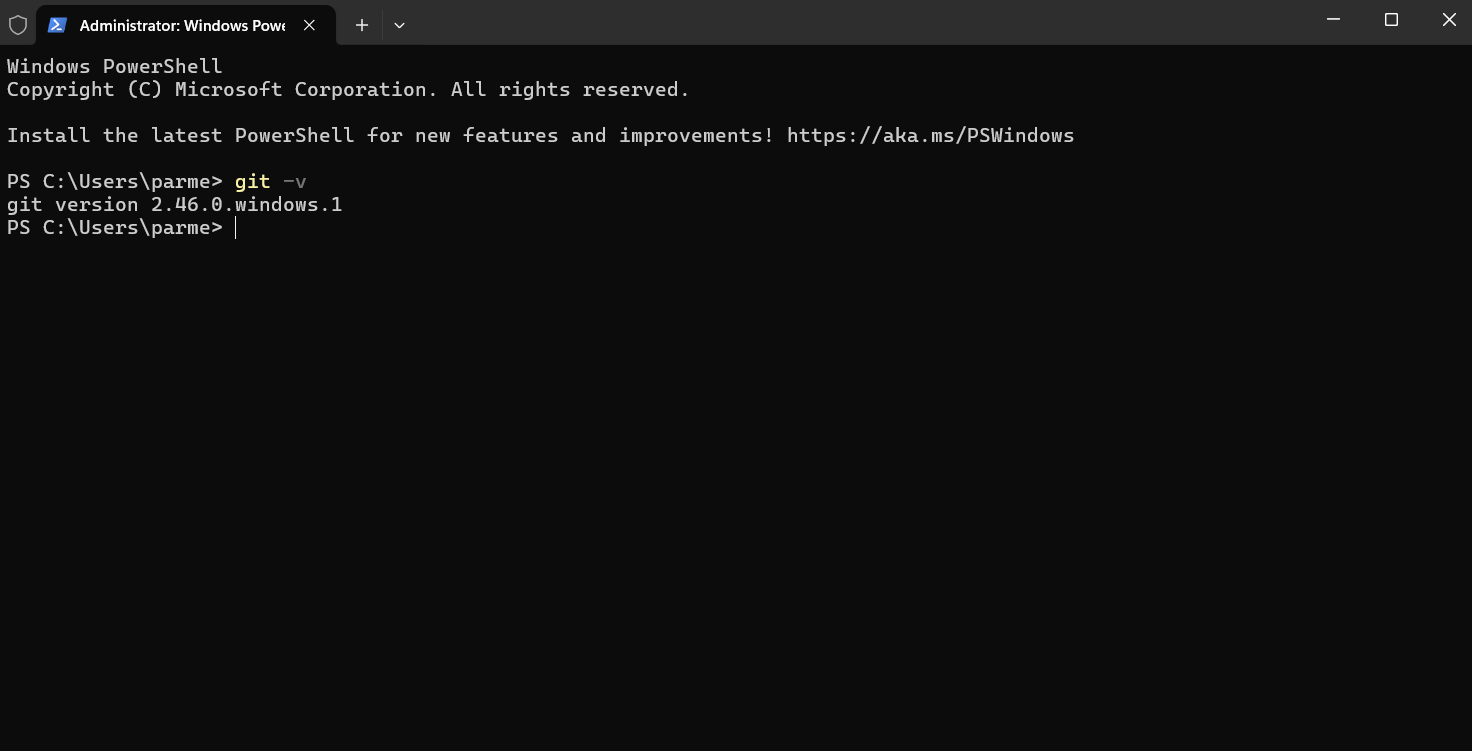
\includegraphics[width=\textwidth]{git-v.png}
    \caption{git -v response example.}
    \label{git-v}   
\end{figure}

If not, try restarting the computer so that Git is added to the Windows PATH variable, which lets Windows know what the \emph{git} command means. If this also doesn't work, Git must be added to the PATH manually. This is annoying and should not really happen but let me know if it does so that I can add instructions.

\subsection{GitHub}

Opening a GitHub account should be as straightforward as opening any account in any other service if you select ``Sign Up'' from 

\url{https://github.com/}


\section{Usage}

\subsection{Starting a new Git repository}

There are two ways to initiate a new Git repository.

\begin{enumerate}
    \item \textbf{Initiate a new Git repository for an existing local folder:} Suppose you have the folder \emph{mvc-self-learning-module} somewhere on your computer and it is not already associated with a git repository. In order to initiate one, you can open the folder in a terminal (can be done by navigating within the folder, and then Right Click $>$ Open in Terminal) and typing the command: 

    \texttt{git init}

    You can visually inspect the Git repository if you have the option of seeing the hidden files on your computer (can be done within the File Explorer itself from View $>$ Show $>$ Hidden Items (\Cref{hidden_items})). In that case, a folder named \emph{.git} should appear in the current directory, which shows that the directory is now a git repository (first folder in \Cref{hidden_items}).

    \begin{figure}[htbp]
        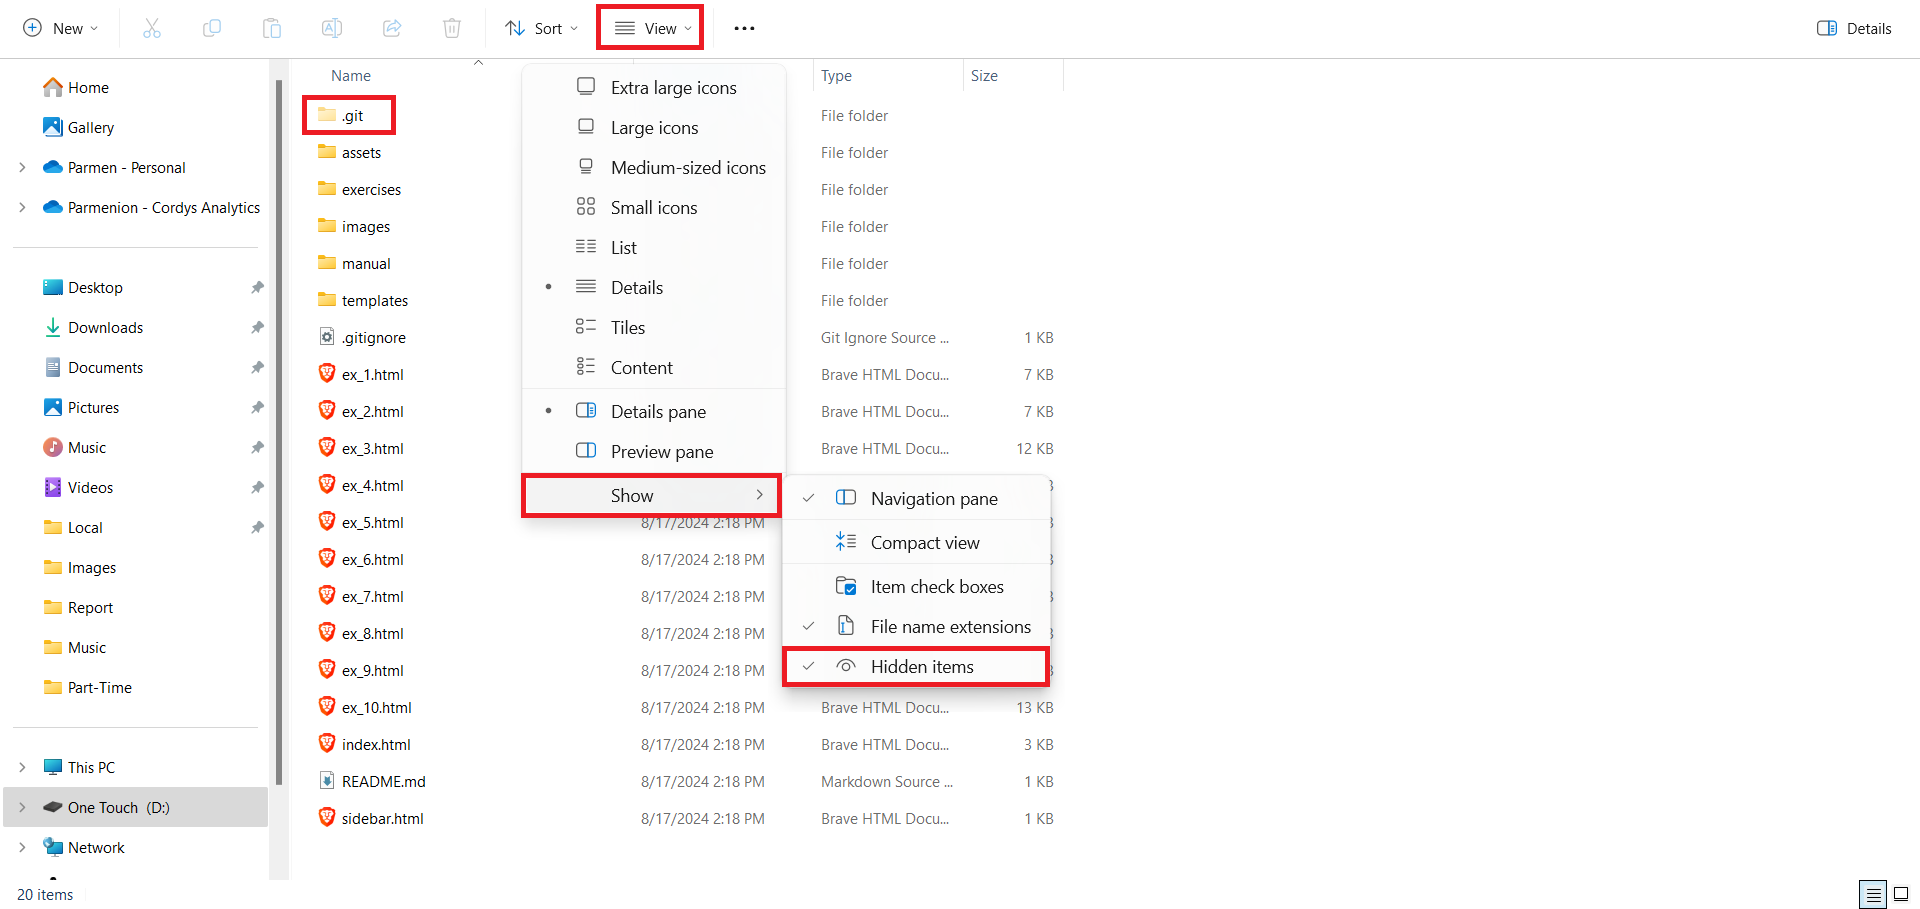
\includegraphics[width=\textwidth]{hidden_items.png}
        \caption{Enable hidden items.}
        \label{hidden_items}   
    \end{figure}

    \item \textbf{Clone an already existing Git repository from GitHub:} This can be done as follows:
    \begin{enumerate}
        \item Find the GitHub repository using your browser.
        \item Copy the link to the repository, e.g.\ \url{https://github.com/StefanMaubach/mvc-self-learning-module}.
        \item Navigate to the location on your computer where you would like to store the repository, and type the command:
        
        \texttt{git clone https://github.com/StefanMaubach/mvc-self-learning-module}
    \end{enumerate}
    The repository should then appear in a new folder named \emph{mvc-self-learning-module} in the desired location.
\end{enumerate}




\end{document}